\setcounter{secnumdepth}{1}
\section{Einführung}
Diese Bachelorarbeit behandelt die Ausführung und Verarbeitung von asynchronen Prozessen in der Programmierung speziell in der Sprache Typescript.\\
Zielgruppe dieser Arbeit sind Personen, die Grundkenntnisse in der Sprache Javascript/Typescript vorweisen können.
Sollte man von der Skriptsprache Typescript noch nicht/kaum etwas gehört haben, sollte vor dem Lesen dieser Arbeit die Offizielle Dokumentation von Microsoft durchgegangen werden.

\begin{center}
\url{https://www.typescriptlang.org/docs/home.html}
\end{center}

In dieser Arbeit wird nur oberflächlich auf die Unterschiede der beiden Sprachen eingegangen. Des Weiteren sollte man von den Kernkonzepten der Promises und Observables schon mal gehört haben, da diese in der Arbeit gegenübergestellt werden.

\subsection{Typescript}
Typescript. Bereits der Name sagt schon was diese Sprache ausmacht. Sie \textit{(\glqq{}Type\grqq{} zu deutsch: Typ)} ist eine typisierte Form der Skriptsprache Javascript. In Typescript ist es Standard, jede Variable, Funktion und Funktionsparameter im Vorfeld zu typisieren. Mit dem Typescript Compiler werden Dateien mit dem Suffix *.ts in *.js überführt. Zur Laufzeit werden Fehler im Code vom Typescript-Compiler entdeckt.

\subsubsection{Beispiel}

\begin{figure}[h!]
\begin{lstlisting}
class Greeter {
    greeting: string;
    constructor (message: string) {
        this.greeting = message;
    }
    greet() {
        return "Hello, " + this.greeting;
    }
}  
\end{lstlisting}
\caption{Typescript Klasse \cite{typescript-example}}
\end{figure}

Im oberen Code-Schnipsel wurden die variablen und die Klassenmethoden nach Typescript-Standard deklariert. Diese Typen werden beim übersetzen in Javascript ignoriert. Der Kompiler einer Entwicklungsumgebung prüft dann, ob beim übergeben eines Parameters in den Konstruktor ein numerischer oder Boolean-Wert eingesetzt wird. Dies wird dann als ein Fehler erkannt. Der Kompiler übersetzt auch nicht direkt deklarierte Typen. Wie in diesem Fall wird erkannt, dass die Methode greet() einen String-Wert zurückgibt.

\begin{figure}[t]
\begin{lstlisting}
var Greeter = (function () {
    function Greeter(message) {
        this.greeting = message;
    }
    Greeter.prototype.greet = function () {
        return "Hello, " + this.greeting;
    };
    return Greeter;
})(); 
\end{lstlisting}
\caption{Überführung in Javascript \cite{typescript-example}}
\end{figure}
In der vom Kompiler auf Javascript übersetzten Version werden die erstellten Klassen und Typen vollständig eliminiert. Was verbleibt ist die Übersetzung der Klassen-Methode greet() und des Konstruktors in einer Funktion. Sowohl Klassen als auch Interfaces werden in Javascript nicht genutzt.
\\\\
Da Syntaktisch alles was auf Javascript geschrieben auch valider Typescript Code ist, kann man Typescript als Superset von Javascript bezeichnen.
Wichtig zu erwähnen ist, dass diese Sprache optionale statische Typen, Klassen und Interfaces bietet, diese sind jedoch keine Pflicht in der Anwendung. Es ist lediglich eine Konvention.
Nichtsdestotrotz findet Typescript immer mehr Beliebtheit in Unternehmensprojekten. Entwicklerteams können durch die Typisierung schneller Bugs am Code erkennen und durch den modularen Aufbau, den Typescript ermöglicht, die Organisation und Dokumentation von großen Projekten verbessern. Diese Tendenz wird von der beliebten Entwicklerplattform Stackoverflow untermauert, die laut einer Umfrage welche die beliebtesten Programmiersprachen unter Entwickler sei, folgendes rauskam:

\begin{figure}[H]
\centering
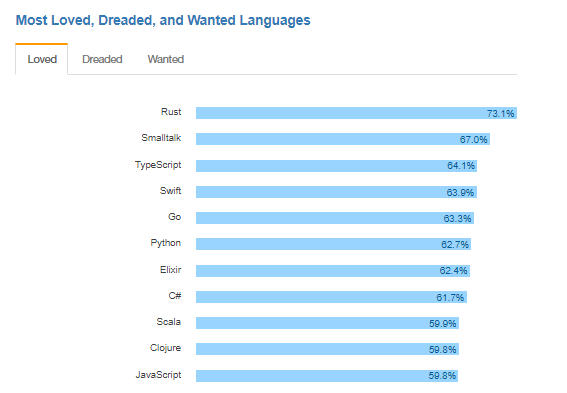
\includegraphics[height=6cm]{stackoverflow-typescript-popularity}
\caption{Prozentualer Anteil der Entwickler die Interesse an neuen Technologien zeigen und weiter mit neuen Technologien arbeiten möchten. \cite{typescript-survey}}
\end{figure}

\subsection{Tooling}

Um unser Typescript-Beispielprojekt modular zu gestalten, brauchen wir die Hilfe eines sog.\glqq Module-Bundlers\grqq{}. Code-splitting und die Unterteilung in Module wollen wir aus dem Grund der Übersichtlichkeit sowie der einfachen Verwaltung des Codes machen. Es ist eine klassische Programmierpraxis, bekannt aus den Programmiersprachen wie C, C++, PHP, Java, usw. Das Problem bei kompiliertem Javascript in einem Internetbrowser ist, dass es nativ kein Code-splitting unterstützt. Alle Skripte werden im Rahmen eines Kontextes im Browser bearbeitet, in der Reihenfolge, in der sie aus einem HTML-Format eingefügt werden. Und hier kommt Webpack ins Spiel. \cite{webpack-einfuehrung}
\\\\
Webpack bearbeitet modular geschriebenen Code und baut darauf einen Dependency-Graphen auf. Alle JavaScript-Module sind darin enthalten und diese in ein (oder mehrere) Bundle gepackt. Dabei kommen zwei Fragen auf:

\subsubsection{Was sind Javascript Module?}
JavaScript-Module ermöglichen es, Code zu gruppieren (auch \glqq{}Splitting\grqq{} genannt), so wie wir, es wie oben erwähnt, aus anderen Programmiersprachen kennen. Das ermöglicht beim überarbeiten des Codes eine bessere Einfindung und Übersicht. Zur Verdeutlichung nehmen wir ein einfaches Beispiel aus unserem Beispielprojekt:


\begin{figure}[H]
\begin{lstlisting}
// views/register-panel.ts
export function createRegisterPanel(): string {
    return `<form id="registerForm" class="sign-up-form mt-5">
                <img class="mb-4" id="hm-logo" width="250" height="auto">
                <div class="text-center">
                    <h1 class="h3 mb-3 font-weight-normal">Register</h1>
                </div>
                <label for="inputEmail" class="sr-only">Email address</label>
                <input type="email" id="inputEmail" class="form-control" placeholder="Email address" required="" autofocus="">
                <label for="inputPassword" class="sr-only">Password</label>
                <input type="password" id="inputPassword" class="form-control mt-1" placeholder="Password" required="">
                <button id="registerButton" type="button" class="btn btn-lg btn-primary btn-block mt-2 mb-3">Sign up</button>
            </form>`;
}
\end{lstlisting}
\end{figure}
In der Datei views/register-panel.ts definieren wir eine Funktion createRegisterPanel(), die HTML-Elemente zurückgibt. Diese Funktionen exportieren wir. Somit ist register-panel.ts unser Modul.

\begin{figure}[H]
\begin{lstlisting}
import {createRegisterPanel} from './views/register-panel';

class Register {

    constructor() {
        document.body.innerHTML = createRegisterPanel();
    }
    
}
\end{lstlisting}
\end{figure}

Unser Modul verwenden wir dann in der Datei main.js, welche die Funktion createRegisterPanel() aus dem Modul importiert und verwendet. Nun können wir mit diesen Dateien in unserem Browser noch nicht viel anfangen. Wir brauchen hier einen Module Bundler wie Webpack, um aus dem Code ein Bundle zu machen.

\subsubsection{Was ist ein Bundle?}

Ein Bundle ist quasi der zusammengefasste JavaScript-Code. Wir geben Webpack als Eingabe unsere Datei main.js, Webpack lädt unsere vollständige Anwendung und erstellt dann – im einfachen Fall – eine JavaScript-Datei, die unseren vollständigen Code enthält und so auch im Browser verwendet werden kann.\cite{Webpack-basics}

\begin{enumerate} 
\item Motivation hinter der Bachelorarbeit
\item Was kann man aus dieser Bachelorarbeit "gewinnen"?
\end{enumerate}

\section{Vorbereitung}
\begin{enumerate} 
\item Welches Framework wird verwendet (Wenn überhaupt?) und welche Sprache angewandt?
\item Repo-Referenz
\end{enumerate}

\subsection{Einführung in asynchrone Operationen}
*Source-code Beispiel*